\section{Definitions and Methods}


\subsection{Definition of fairness}
There are in general two types of fairness in related literatures: the first is individual fairness, which is based on the belief that similar individuals should be treated similarly. The other is group fairness, which states members from different groups should have similar chance to achieve target outcomes. In this project, we narrow our scope to group fairness. Following the idea of group fairness \cite{hardt2016equality, dwork2012fairness, feldman2015certifying}, suppose for the $i^{\text{th}}$ protected group, the classification accuracy is $\alpha_i$, then we define the unfairness in classification tasks as
\begin{equation}
UF := \text{Var}(\alpha_i)
\end{equation}
It's straightforward to interpret $UF$ as the divergence of accuracies among all the protected groups. The closer their accuracies are, the smaller $UF$ is.

\subsection{Non-deep learning baseline - Logistic Regression}
The hyperparameters of our logistic regression model are as follows:
\begin{itemize}
    \item Loss function: CrossEntropyLoss
    \item Optimizer: SGD
    \item Learning rate: 0.001
    \item Number of epochs: 30
\end{itemize}

\subsection{Deep learning baseline (1) -  FeedForward Neural Network}
The hyperparameters of our FeedForward model are as follows:
\begin{itemize}
    \item Structure: 2 fully connected linear layers, followed by ReLU and BatchNorm1d
    \item Loss function: CrossEntropyLoss
    \item Optimizer: Adam
    \item Learning rate: 0.001
    \item Number of epochs: 20
\end{itemize}


\subsection{Deep learning baseline (2) -  Convolutional Neural Network}
The hyperparameters of our CNN model are as follows:
\begin{itemize}
    \item Structure: 3 convolutional layers followed by a fully connected linear layer (See Figure 1)
    \item Loss function: CrossEntropyLoss
    \item Optimizer: Adam
    \item Learning rate: 0.001
    \item Number of epochs: 10
\end{itemize}

\begin{figure}[H]
	\centering
	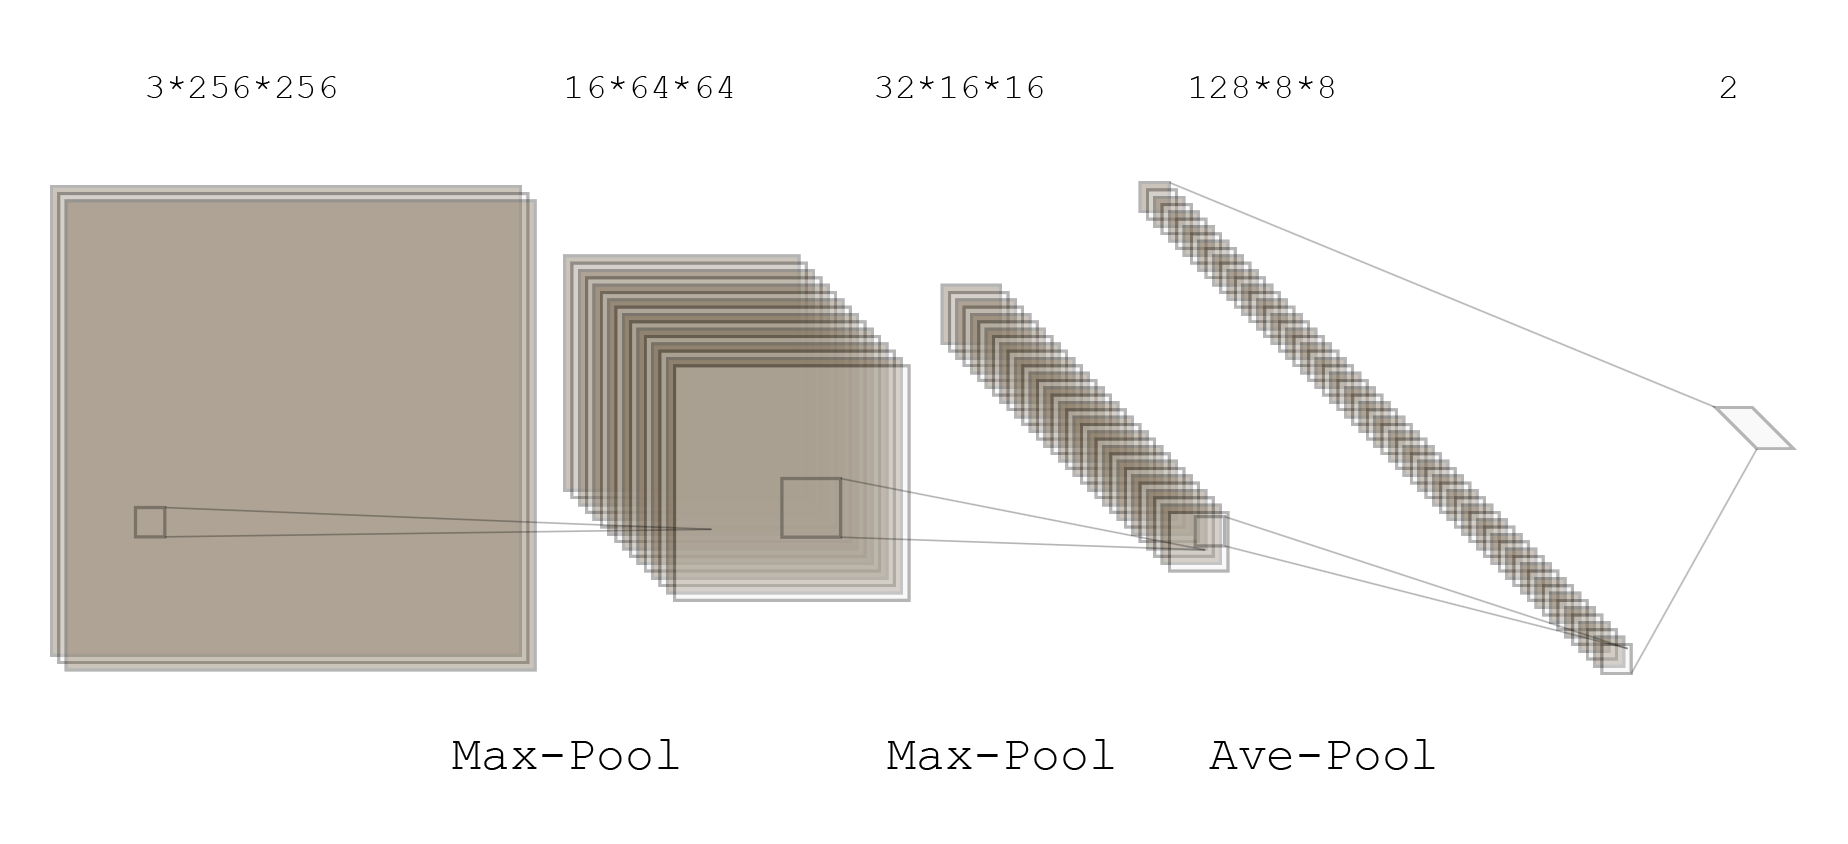
\includegraphics[width=0.8\textwidth]{figure/CNN.png}
	\caption{CNN baseline structure}
	\label{fig: cnn-structure}
\end{figure}


\subsection{Deep learning baseline (3) - Residual Network}
The hyperparameters of our ResNet model are as follows:

\begin{itemize}
    \item Structure: ResNet-34
    \item Loss function: CrossEntropyLoss
    \item Optimizer: Adam
    \item Learning rate: 0.0001
    \item Number of epochs: 30
\end{itemize}

\subsection{Novel approach (1) - Regularized ResNet}
We propose a regularized ResNet. Our basic idea is to update the loss function by adding a $UF$-based regularization (penalty) term:

\begin{equation}
\mbox{New Loss} = \mbox{CrossEntropyLoss} + w*\mbox{Penalty} 
\end{equation}

Here, $w$ is a coefficient of the penalty term. In the process of tuning a model, we find a critical issue when we assign a value to $w$ that is too large.  That is, while $UF$ becomes smaller than the baseline $UF$s, the validation accuracy soon drops and converges to around 50\%, or random chance.  Hence, we use a step decay, i.e. $w = \delta(\mbox{step})$, to mitigate the decrease in loss as training occurs. The formula for step decay is as follows

\begin{equation}
\delta(\mbox{step}) = w_{start} - \frac{\mbox{step}}{N_{steps}}(w_{start} - w_{end}),
\end{equation}

where $N_{steps}$ is the total number of steps and $w_{start}$ and $w_{end}$ are the starting (maximum) and ending (minimum) weights for the penalty term, respectively. We set $(w_{start}, w_{end}) = (1, 0.001)$.

We also find that "MiddleEastern" has an exceptionally higher accuracy compared to the accuracies of other ethnic groups.  Hence, we apply a weight 10 to "MiddleEastern" the penalty function, i.e.

$$
{\mbox{Penalty} = 10*(acc_{\mbox{MiddleEastern}} - acc_{\mbox{average}})^2 + \sum_{i\in \{\mbox{other ethnicities}\}} (acc_{\mbox{i}} - acc_{\mbox{average}})^2}
$$,

where $acc_{\mbox{MiddleEastern}}$ and $acc_{\mbox{average}}$ are the validation accuracy of gender among Middle Eastern faces
\\
and average validation accuracy amongst all ethnic groups, respectively. 

The hyperparameters of our regularized ResNet model are as follows:
\begin{itemize}
    \item Structure: ResNet-34
    \item Loss function: CrossEntropyLoss
    \item Optimizer: Adam
    \item Learning rate: 0.0001
    \item Number of epochs: 30
\end{itemize}

\subsection{Novel approach (2) - Fair Masking}
We also propose fair masking, which is another novel approach to mitigate the bias of neural networks. The general idea is that we focus on one hidden layer of the network and regularize the values of all neurons strongly dependent with the protected feature. 

Our model is based on convolutional neural network, in which we specify a hidden layer $\mathcal{H}$. Suppose there are $K$ neurons in $\mathcal{H}$ and the value passed from previous layer is $V = \{v_1, \dots, v_K\}$. We add a mask $M = \{m_1, \dots, m_K\}$ on previous output at $\mathcal{H}$, then pass them to the next layer. That is, the value restored in $k^{\text{th}}$ neuron is 
$$
m_k \odot v_k.
$$
Initially, all the $m_k$ are set to be 1. This implies that the training process of this fair-masked CNN is the same as a normal CNN. After the training process, we record all the $V$s, since for each image $X_i$, we can have a corresponding $V_i$ by simply inputting image into the network. We select those $v_k$ ($k \in \{1, \dots, K\}$) that are strongly dependent with the protected features and set the corresponding $m_k = 0$. After this masking process, we obtain the final fair-masked CNN.

However, the correct dependence test can be hard to find. The two protected groups we chose are gender and ethnicity, both of which are categorical, whereas the hidden features in the network are all continuous . There is no widely used test for the dependence between a non-binary categorical variable (ethnicity in our case) and a continuous variable. Hence, we proposed two novel approaches to tackle this problem: a correlation-based test and a logistic regression-based test.

\subsubsection*{Correlation-based dependence test}
In this test, we need an additional validation set. When training is complete, we calculate the classification accuracy of the network on this validation set. Then, we rank all the protected features in a ascending order according to classification accuracy.
\\
\\
For example, in the gender classification task, we specify the ethnicity as protected group, in which there are seven classes. For each class, we can calculate the classification accuracy of gender and rank all of the accuracies in an ascending order. Then, we assign a value $R_c$ to each class which equals to its ranking (e.g. if the class ``Latino'' has the highest classification accuracy among the seven classes, it would have a value $R_c = 7$, and if ``White'' has the lowest accuracy, it would have value $R_c = 1$). Then, we can calculate the correlation between $R_c$ with each hidden feature. As a result, we would apply the threshold $T_c$ on the correlation and update the value of masks by:
\begin{equation}\label{correlation}
m_k = \mathbf{1}\{|\text{Cor}(v_k, R_c)| < T_c\}.
\end{equation}

\subsubsection*{Logistic regression-based dependence test}
As an alternative approach, we propose to fit a logistic regression to test the dependence between hidden features and protected ones. Recall that for multi-class logistic regression, if we have $\mathcal{S}$ classes in total, then we have
$$
\mathcal{P}(Y_i = s) \propto \exp{(-X_i\beta_s)},
$$
where $X_i = \{X_{i,1}, \dots, X_{i,K}\}$, $\beta_s = \{\beta_{s,1}, \dots, \beta_{s,K}\}^{\top}$ and $\beta_0 = \{0, \dots, 0\}^{\top}$. This implies that for the $k^{\text{th}}$ feature, there will be $\mathcal{S} - 1$ associated coefficients, namely $\{\beta_{1,k}, \dots, \beta_{\mathcal{S},k}\}$. Once we fit a logistic regression, we assign a value $R_l := \max_i\beta_{i,k} - \min_i\beta_{i,k}$. We sort all $K$ features using $R_l$ and select top-$T_l$ features to mask out.

In the context of gender prediction with ethnicity as protected group, psuedocode for a fair-masked CNN is shown in Algorithm \ref{alg: 1}.

\begin{algorithm}[H]
	\KwData{Facial images}
	\texttt{Network}: A Convolutional Neural Network with a pre-specified hidden layer $\mathcal{H}$ for fair masking
	
	\KwResult{Classification result}
	Set $m_i = 1$ for $i \in \{1, \dots, K\}$
	
	\While{training}{
		\ normally train the network
	}
	Conduct dependent test to identify relevant features $\{s_1, \dots, s_k\} \subseteq \{1, \dots, K\}$ that are strongly associated with the protected features.
	
	Set $m_i = 0$ for $i \in \{s_1, \dots, s_k\}$.
	
	\While{prediction}{
		\ calculate $V = (v_1, \cdots, v_K)$, the values passed to layer $\mathcal{H}$ \\
		use $\{m_k \odot v_k\}_{k=1}^K$ as input and forward the network from $\mathcal{H}$
	}
	\caption{\texttt{Fair-Masked CNN}}
	\label{alg: 1}
\end{algorithm}

The hyperparameters of our fair-masked CNN model are as follows:
\begin{itemize}
    \item Structure: see Figure 2 (number of hidden features changes for value of $T_c$)
    \item Loss function: CrossEntropyLoss
    \item Optimizer: Adam
    \item Learning rate: 0.001
    \item Number of epochs: 10
\end{itemize}

Correlation-based test: We set $T_c$ at values between 0.3 and 0, to select 1 to total 32 hidden features.

Logistic regression-based test: We set $T_l$ at values between 1 to 32, to select 1 to total 32 hidden features.

\begin{figure}[H]
	\centering
	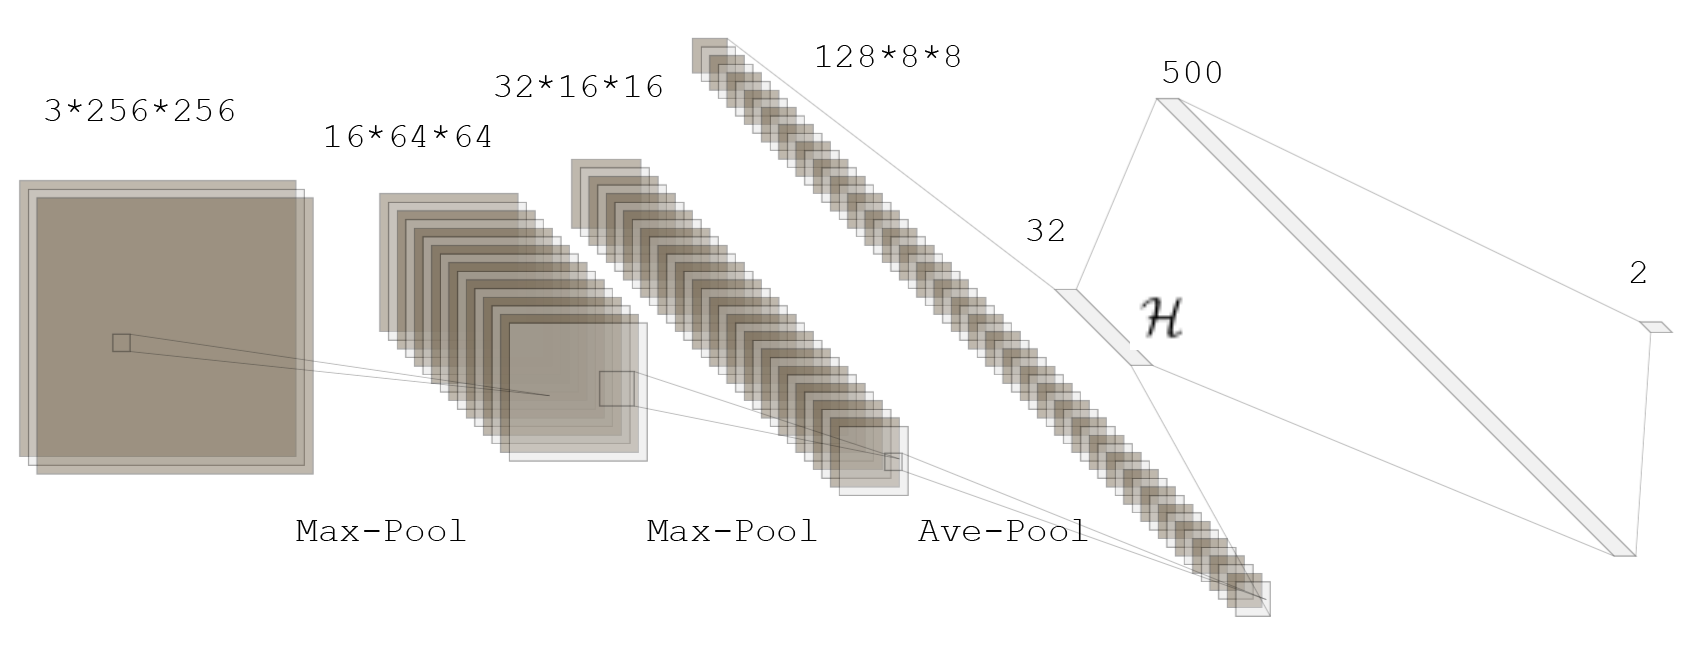
\includegraphics[width=0.8\textwidth]{figure/fairmaskedCNN.png}
	\caption{Fair Masked CNN}
	\label{fig: fairmaskedcnn-structure}
\end{figure}


\subsection{Novel approach (3) - Transfer Learning}

Finally, we propose transfer learning from the ResNet-34 baseline model trained on FairFace onto the cleaned IMDb-Faces dataset. Simply put, the IMDb data is tested on the pretrained ResNet model. The IMDb dataset differs from FairFace in that it relatively larger and much more imbalanced with respect to gender and ethnicity classes.

Given a source domain $D_S$ and a corresponding source task $T_S$, as well as a target domain $D_T$ and a target task $T_T$, the objective of transfer learning is to learn the target conditional probability distribution $P(Y_T | X_T)$ in $D_T$ with the information gained from $D_S$ and $T_S$, where $D_S$ \neq $D_T$ and $T_S$ \neq $T_T$. 

Knowing that domain $D=\{X,P(X)\}$ and target $T=\{Y,P(Y)\}$, in our transfer learning scenario, we have $P(Y_S | X_S)$ \neq $P(Y_T | X_T)$. This means that the conditional probability distributions of the source and target tasks (where source refers to FairFace and target refers to IMDb) are different, due to the differences in class balance \cite{ruder_2019}.